
%--------------------------------------------------------------------
%--------------------------------------------------------------------
% Formato para los talleres del curso de Métodos Computacionales
% Universidad de los Andes
%--------------------------------------------------------------------
%--------------------------------------------------------------------

\documentclass[11pt,letterpaper]{exam}
\usepackage{amsmath}
\usepackage[utf8]{inputenc}
\usepackage[spanish]{babel}
\usepackage{graphicx}
\usepackage{tabularx}
\usepackage[absolute]{textpos} % Para poner una imagen completa en la portada
\usepackage{hyperref}
\usepackage{float}

\newcommand{\base}[1]{\underline{\hspace{#1}}}
\boxedpoints
\pointname{ pt}

\extraheadheight{-0.15in}

\newcommand\upquote[1]{\textquotesingle#1\textquotesingle} % To fix straight quotes in verbatim



\begin{document}
\begin{center}
{\Large Universidad de los Andes - M\'etodos Computacionales Avanzados} \\
Ejercicio 1 - \textsc{MPI}\\
8-02-2017\\
\end{center}



\vspace{0.3cm}


\noindent
La solución a este ejercicio debe subirse por SICUA antes de las 7:00PM
del viernes 10 de febrero del 2017. 
Los c\'odigos deben encontrarse en un unico repositorio de \verb'github'
con el nombre \verb"NombreApellido_Ej1". Por ejemplo yo deber\'ia
subir crear un repositorio con el nombre
\verb"JaimeForero_Ej1". 

\noindent
En el repositorio deben estar los siguientes elementos.
\begin{itemize}
\item (60 puntos) Un c\'odigo fuente en C paralelizado en MPI que resuelve las ecuaciones diferenciales y produce datos.
\item (10 puntos) Un c\'odigo en Python que lee los datos producidos por el
  c\'odigo en C y produce visualizaciones.
\item (10 puntos) Un makefile que compila el c\'odigo en C y produce visualizaciones en Python.
\item (10 puntos) Un script para enviar el c\'odigo al encolador del cluster con $n=4$ procesadores.
\item (10 puntos) Un archivo de texto (\verb"README") con nombres completos y c\'odigos de los integrantes (m\'aximo dos personas).
\end{itemize}

\vspace{0.3cm}

\begin{questions}
\question{\bf{Condensador de placas paralelas}}

Considere un condensador de placas paralelas ubicado en una regi\'on
bidimensional del espacio, de dimensiones $L\times L$. Las placas
tienen un largo $l$ y una separaci\'on $d$ entre ellas, como se
muestra en la figura \ref{fig:gridplates}. 

\begin{figure}[H]
  \centering
  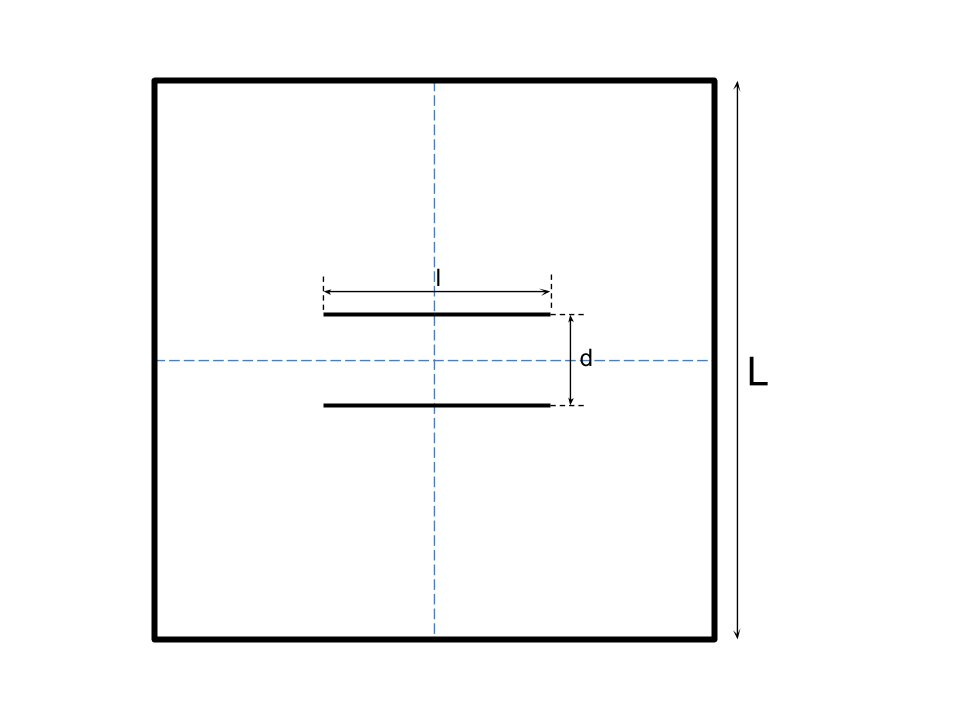
\includegraphics[width=10cm]{gridplates}
  \caption{\label{fig:gridplates} Condensador de placas paralelas.}
\end{figure}

Supongamos que existe una diferencia de potencial constante $V_0$
entre las placas (una de las placas se encuentra a $-V_0/2$ y la otra
a $V_0/2$). Adem\'as, en el borde de la regi\'on tomemos el potencial
fijo en $0$. 

El potencial el\'ectrico $V(x,y)$ en la regi\'on debe cumplir la
ecuaci\'on de Laplace 

\begin{equation*}
 \nabla^2V(x,y) = \frac{\partial^2 V(x,y)}{\partial x^2} +
 \frac{\partial^2 V(x,y)}{\partial y^2}=0. 
\end{equation*}

As\'i mismo el campo el\'ectrico est\'a dado por.
\begin{equation*}
\mathbf{E}(x,y) = -\nabla V(x,y) = \left(-\frac{\partial V(x,y)}{\partial x}, -\frac{\partial V(x,y)}{\partial y}\right)
\end{equation*}

Para calcular el potencial num\'ericamente se debe discretizar la
regi\'on como una matriz de tama\~no $L/h \times L/h$, donde $h$ es la
separaci\'on entre los puntos y utilizar el esquema de diferencias
finitas. 

Escriba un programa en C (\verb"placas.c") que encuentre el
potencial el\'ectrico con el m\'etodo de relajaci\'on usando N
iteraciones. El mismo programa debe calcular el campo el\'ectrico a
partir de la soluci\'on final del potencial.
Escriba un c\'odigo en Python \verb'grafica.py' que grafique el
potencial y el campo el\'ectrico usando \verb'imshow' y
\verb'streamplot' en una grafica llamada \verb'placas.pdf'.

Utilice $L = 5$ cm, $l = 2$ cm, $d = 1$ cm, $h = 5/512$ cm, $V_0 = 100$ V y $N = 2\times (L/h)^2$ iteraciones.
 
\end{questions}

\end{document}

